\documentclass{article}
\usepackage{enumitem}
\usepackage{amsmath}
\usepackage[margin=1in]{geometry}
\usepackage{fancyhdr}
\usepackage{graphicx}

\pagestyle{fancy}
\fancyhf{}
\rhead{CS 535, Mini Project 2}
\lhead{Lixuan Zhu (lz306)}

\begin{document}
\begin{enumerate}
\item
    \begin{enumerate}
    \item
        \begin{itemize}
            \item
                Setting the number of points apriori: K-Means is sensitive to this factor because it assumes there are K clusters in the data set where K is determined apriori. K-Means does not attempt to find the inherent organization of the data but simply finding the most probable clusters according to K.
            \item
                Anisotropy: K-Means is sensitive to anisotropy in data because it assumes the data is spherical/convex. In the K-Means model, it tries to fit data around K centers which minimizes the within cluster sum of squared criterion. If the data in an intuitive cluster is distributed anisotropicly, K-Means is likely to group a part of the data with data from other intuitive cluster to minimize within cluster sum of square instead of preserving the intuitive non-sperical shape.
            \item
                Unequal variance: K-Means assumes the data is separated in K groups of equal variance. In each iteration, K-Means reduces the difference in variance between K clusters and converges until the variance between groups are the same. Thus if two intuitive clusters have different variance, K-Means will compensate by assigning points from other intuitive clusters to each until the variance converges, producing an unsatisfactory cluster assignment.
            \item
                Unequal cluster sizes: K-Means is affected because it tries to minimized the within-cluster sum of squares, which natually put more weight to clusters with more data. Consider a dataset which contains two intuitive clusters $K, J$, where the number of data points in each cluster $k << j$ and the average squared distance to cluster center is the same $d_{avg}$. Then the within-cluster sum of squares $k*d_{avg} << j*d_{avg}$. K-Means will assign points from intuitive cluster $J$ to $K$ in order to balance the within-cluster sum of squares between them, thus producing an undesirable cluster assignment. In the example given by the code, the within-cluster sum of squares are incidentally equal between three intuitive clusters although they have different number of data points, thus K-Means is able to produce a desirable result under such specific condition.
        \end{itemize}
    \item
        As we can see in Figure 1, some points that belongs to the green cluster in the original cluster assignment is marked as red after feature scaling and vice versa. Feature scaling affects the K-Means because it affects the variance and the isotropy of each cluster. In the lower graph of Figure 1, the clusters are less spherical compare to the upper graph, thus K-Means moves points between the red and green clusters to balance the variance between them. Please refer to $simple\_feature\_scaling.py$ for code.
        \begin{figure}[h]
            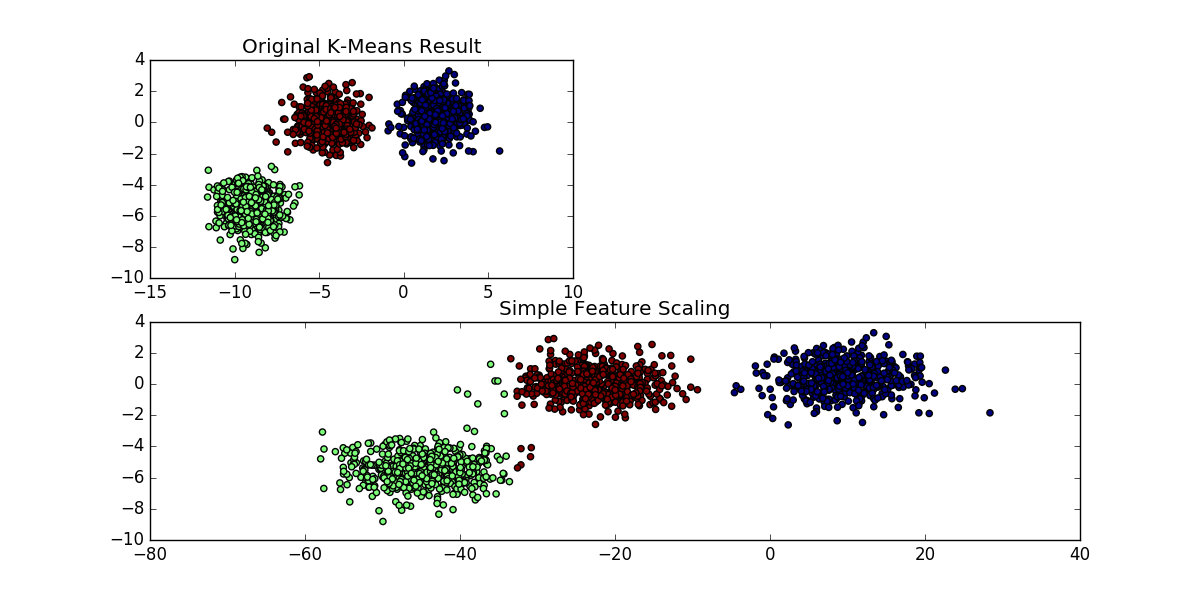
\includegraphics[width=.8\linewidth]{figure_1.png}
            \caption{Before and after increasing the x-feature by a factor of 5.}
            \label{fig:graph1}
        \end{figure}
    \item
    \item
        We can preprocess the data by normalization. Normalize the mean and scale each feature to unit variance.
    \item
        As shown in the upper right graph in Figure 2, GMM mitigates the effect of anistropicy by allowing custom covariance matrices for each Gaussian distribution. As shown in the bottom-left graph in Figure 2, GMM mitigates the effect of unequal variance because it allows each cluster(Gaussian distribution) to have different variances. Although cannot be shown through this dataset, GMM also mitigates the effect of unevenly sized blobs because it allows different covariance matrices for each cluster. Since GMM requires a input of K mixtures apriori, it does not mitigate the effect of setting the number of clusters apriori in K-Means.
        \begin{figure}[h]
            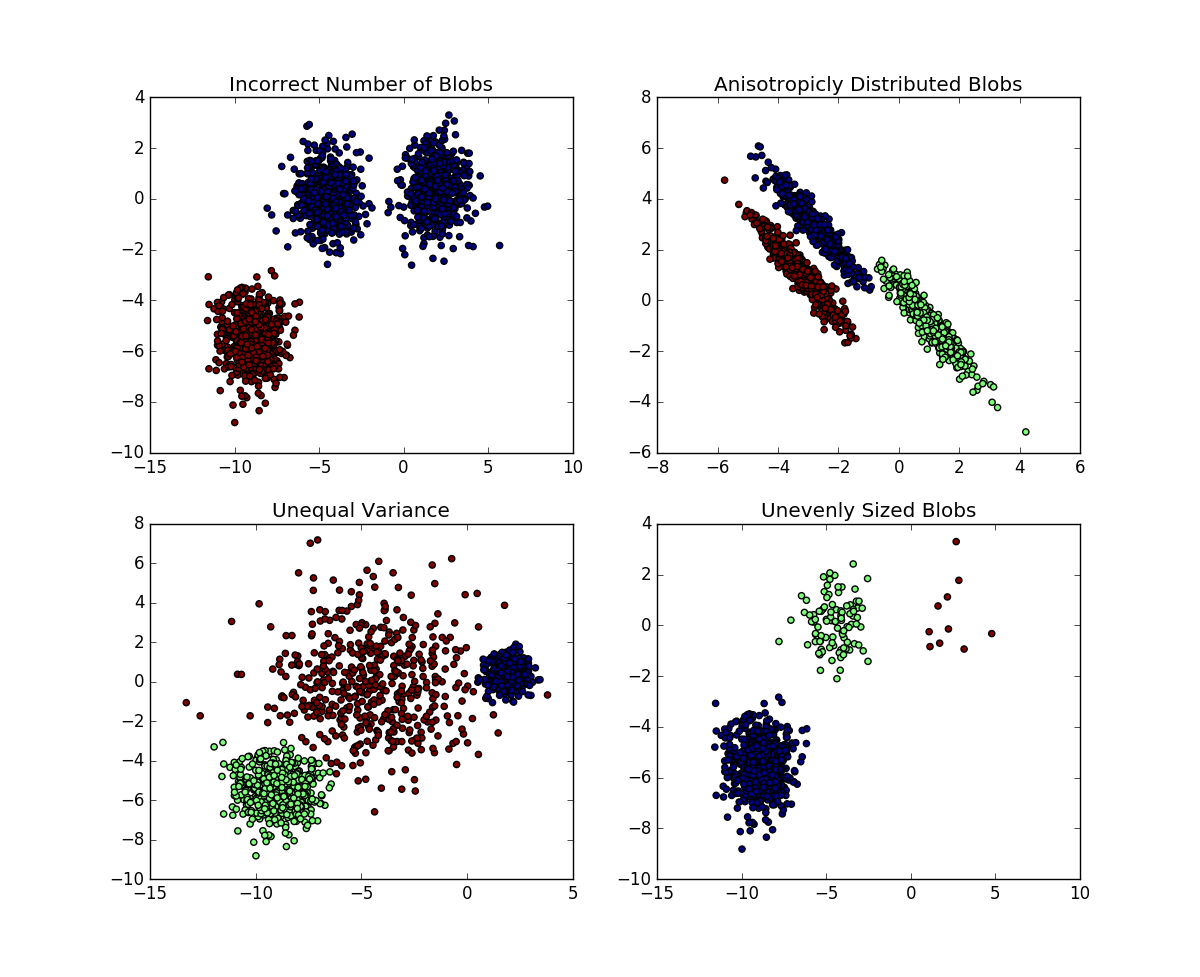
\includegraphics[width=1\linewidth]{figure_2.png}
            \caption{Clustering using GMM.}
            \label{fig:graph2}
        \end{figure}
    \end{enumerate}
\item
    \begin{enumerate}
    \item
        For Gaussian distribution in $d$ dimensions, we have density function:
        \begin{equation} \label{eq1}
            p(x_d) = \frac{1}{\sqrt{(2\pi)^d|\Sigma|}}\exp(-\frac{1}{2}(x - \mu)^T\Sigma^{-1}(x - \mu))
        \end{equation}
        where $\Sigma$ is the covariance matrix and $|\Sigma|$ is the determinant of $\Sigma$. Since we have $\mu = 0$ and $\Sigma = \sigma^2I$, substitute them in (1) we get:
        \begin{equation} \label{eq2}
            p(x_d) = \frac{1}{(2\pi\sigma^2)^{d/2}}\exp(-\frac{||x||^2}{2\sigma^2})
        \end{equation}
        Since the integral of the probability density over a thin shell of radius $r$ and thickness $\epsilon$ is equivalent of the volume of the $d$ dimentional geometric space, we can find the integral of $p(x_d)$ by calculating the volume of the shell $S_dr^{d-1}\epsilon$:
        \begin{equation} \label{eq3}
            p(r|d)\epsilon = \int p(x_d)dx_d \approx p(r)S_dr^{d-1}\epsilon\\
        \end{equation}
        Since $||x||^2 = r^2$, substitute $r$ into (2) we have:
        \begin{equation}
            p(r|d)\epsilon = \frac{S_dr^{d-1}}{(2\pi\sigma^2)^{d/2}}\exp(-\frac{r^2}{2\sigma^2})\epsilon
        \end{equation}
        which is what we wanted to show.
    \item
    \item

    \item
    \item
    \item
    \end{enumerate}
\item
    \begin{enumerate}
    \item
    \item
    \end{enumerate}
\end{enumerate}
\end{document}
